\chapter{Semileptonic final state}
\label{cap6}

\textit{In this chapter is described   the search for high mass spin-0 resonances in the semileptonic final state. In this mass regime the hadronically decaying boson may be sufficiently boosted that its decay products are contained in a single jet, thus merged jet
reconstruction and substructure techniques are utilised. The case where the hadronic
decay products are resolved is also considered. I have contributed in the synchronisation (in terms of signal modelization, uncertainties, 
backgrounds estimation, etc.) among the fully- and the semi-leptonic analysis. }

\section{Overview of the semi leptonic analysis}
The $X \to WW \to \ell \nu q \bar{q}$ final state is one of the dominant decay channel of a SM-like Higgs boson for masses above 200 GeV,  Fig.~\ref{BRTotalUncertBands4f2} in green.
In the mass regime of interest the hadronically decaying boson may be sufficiently boosted that
its decay products are contained in a single merged jet. Jet substructure techniques are used
to identify merged jets with two well defined subjets and to determine the merged jet mass,
helping to discriminate vector boson decays from QCD jets coming from quarks and gluons. If
the hadronic decay products are resolved then the boson decay may be reconstructed as two
quark-jets (a dijet). In this analysis it is first attempted to reconstruct boson candidates using
merged jets, if no boosted candidates are found then dijet reconstruction is attempted.
The leptonically decaying boson is reconstructed as a single isolated lepton and missing transverse energy
orresponding to the neutrino. An estimate of the neutrino longitudinal
momentum is derived by imposing the constraint of the W mass on the invariant mass of the $\ell \nu$ system.
The dominant background processes
are from $W$+jets and top production, with a smaller contribution from diboson, $Z$+Jets and
QCD multijet events. Unlike for the signal the mass distribution of the background events is
not resonant, providing a useful handle to isolate signal events. Data from signal-free control
regions are used to normalize and tune the W+jets and top MC background prediction reducing
the dependence on the simulation.
The kinematic information of the final state particles is fully exploited with the use of a matrix
element based kinematic discriminant to enhance the sensitivity to signal. Identifying addi-
tional jets in the event also leads to increased sensitivity to signal produced through vector-
boson fusion. Effects due to the interference between the signal, the SM Higgs boson and
the WW continuum background are also considered.

\section{Jets for Boosted and Resolved selection}
Hadronic jets are reconstructed with the anti-$k_T$ clustering algorithm  using two different
radius parameters, $R = 0.8$ (AK8) and $R = 0.4$ (AK4). The AK8 algorithm is adopted for
reconstructing the hadronic W decay in a single merged jet when the decay products are highly
collimated, while the AK4 algorithm is used to reconstruct the hadronic W decay when the
decay products are resolved.
Charged Particle Flow
constituents not associated to the primary vertex are not used in the jet clustering procedure.
To avoid double counting of the same object
reconstructed in different collections, jets are required to be separated from the selected isolated
leptons by $\Delta R(lj)> 0.8 $ for AK8 jets by  $\Delta R(lj)> 0.4$ for AK4 jets.
For the selection of $W$ candidates is require two AK4 jets both with $p_T>30$ GeV or an AK8 jet with  $p_T>200$.
The final hadronic $W$ candidate requirements for the merged and resolved analyses
will be discussed in detail in the following.
This analysis also makes use of the n-subjettiness variable~\cite{Thaler:2011gf}  to quantify the compatibility
of AK8 jets with a substructure hypothesis of n-subjets. It is based on the distribution of the
jet constituents with respect to the subjet axes. The ratio of 2-subjettiness and 1-subjettiness,
 $\tau_2 /\tau_1$, allows the dipole structure of hadronic W decays to be distinguished from the monopole
structure of QCD jets.
In order to mitigate the effect of pileup on the jet substructure observables used in this analysis
(softdrop mass and n-subjettiness) the pileup per particle identification (PUPPI)~\cite{Bertolini2014} method is
implemented.

\subsection*{Boosted selection}
For the boosted merged jet analysis an AK8 jet with corrected PUPPI softdrop mass $m_J >$ 40 GeV is required.
To suppress the background from QCD multijet events it is require $MET>40$ GeV.
The $W \to \ell \nu$ and $W \to q \bar{q}$ decay candidates satisfying the boosted analysis requirements are combined into $\ell \nu J$ resonance candidates.
To suppress the dominant $W+$jets background, candidates are selected in the PUPPI softdrop mass region  $65<m_J < 105$, that is the signal region (SR).
Outside of this signal region,i.e. in a mass range  $65<m_J < 105$,the candidates are used for background determination (or sideband region) (SB).
A top-enriched control region (Top CR) is also defined by reversing the b-veto and requiring at least one AK4
b-tagged jet in the event.
For the final selection a cut on the PUPPI n-subjettiness ratio $\tau_2 /\tau_1<0.4$ is used to identify boosted
hadronic boson candidates. The entire selection procedure described above is referred to as the ``boosted selection''.
The $m_J$ distribution in SR, SB and Top CR is shown in Fig.~\ref{mJ}.
\begin{figure}
\centering
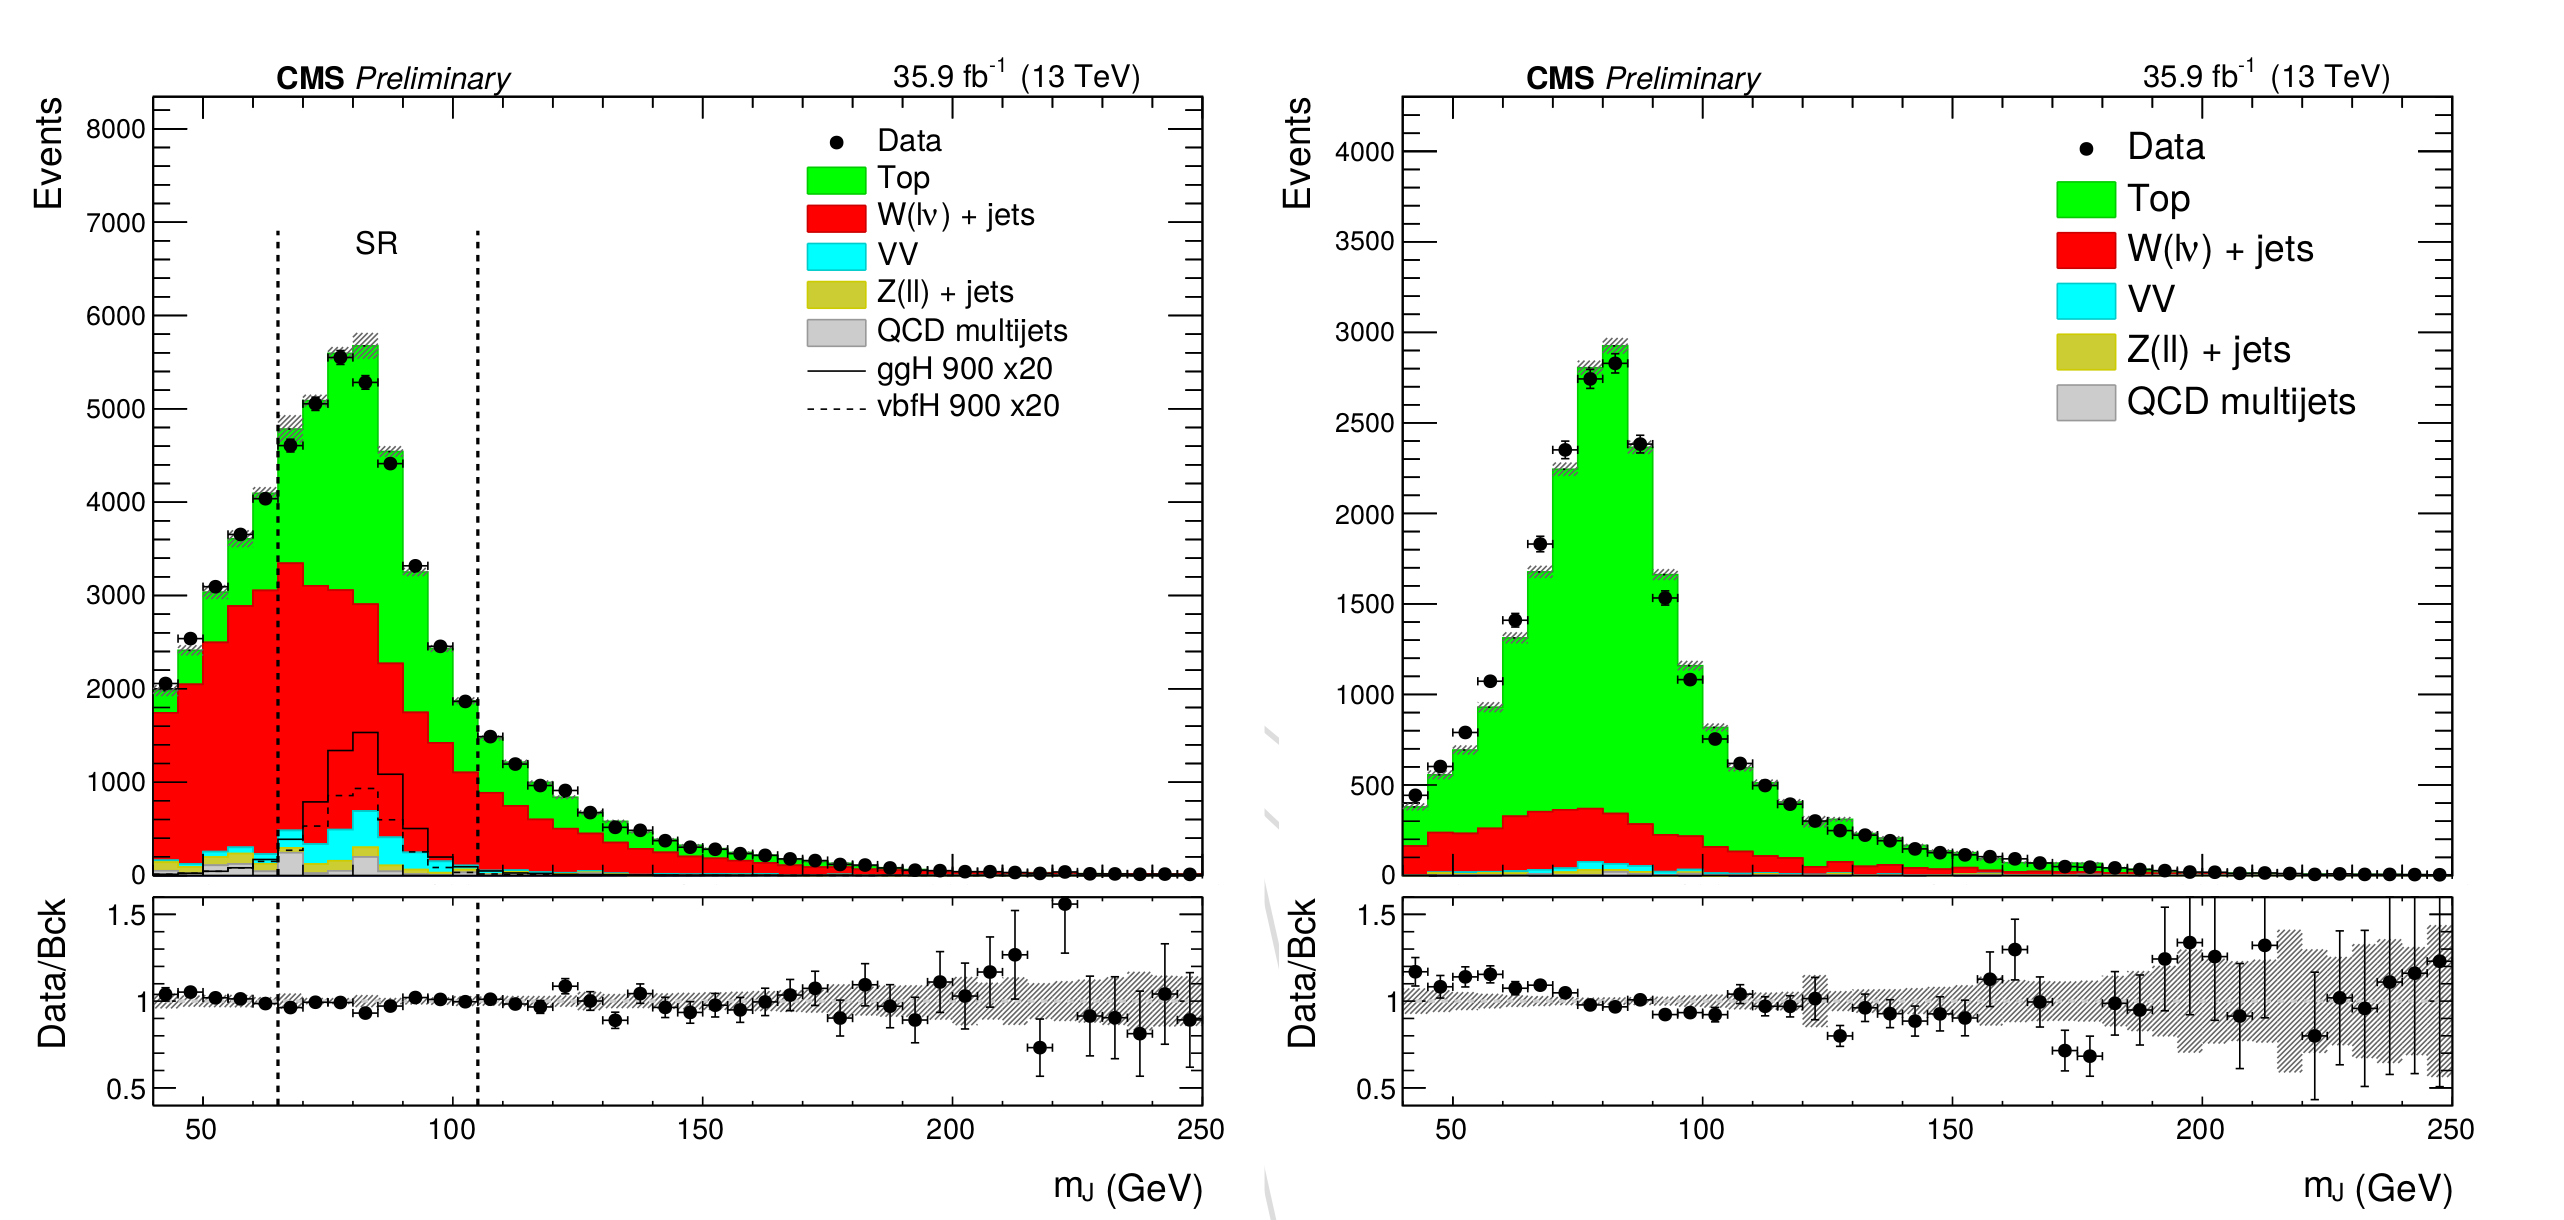
\includegraphics[scale= 0.8]{../Cap5/mJ}
\caption{Hadronic W candidate PUPPI softdrop mass for events passing
the boosted selection in the SR and SB (left), and the Top CR (right).}
\label{mJ}
\end{figure}

\subsection*{Resolved selection}
For events which do not pass the boosted jet selection, it is attempted to reconstruct a resolved
hadronic W decay using two AK4 jets.
A kinematic fit is performed to the dijet system using
the $W$ mass constraint, in events with greater than two jets the dijet pair with the smallest $\chi^2$ is
chosen.
To suppress the background from QCD multijet events we require $MET>$30 GeV and
 $W_{m_T} >$ 50 GeV, where $W_{m_T}$ is the transverse mass of the leptonic W candidate. 
The $W \to \ell \nu$ and $W \to q \bar{q}$  decay candidates satisfying these requirements are combined into $\ell \nu jj$ resonance
candidates. To suppress background $\ell \nu jj$ candidates are selected in the dijet mass signal region (SR)
65 $< m_{jj} <$ 105 GeV. Sideband (SR) and top-enriched control regions (Top CR) used for background estimation are
defined as for the ``boosted selection''.
The entire selection procedure described above is referred to as the ``resolved selection''.
The $m_{jj}$ distribution for events passing the resolved selection in SR,  SB and  Top CR is reported in Fig.~\ref{mjj}.
\begin{figure}
\centering
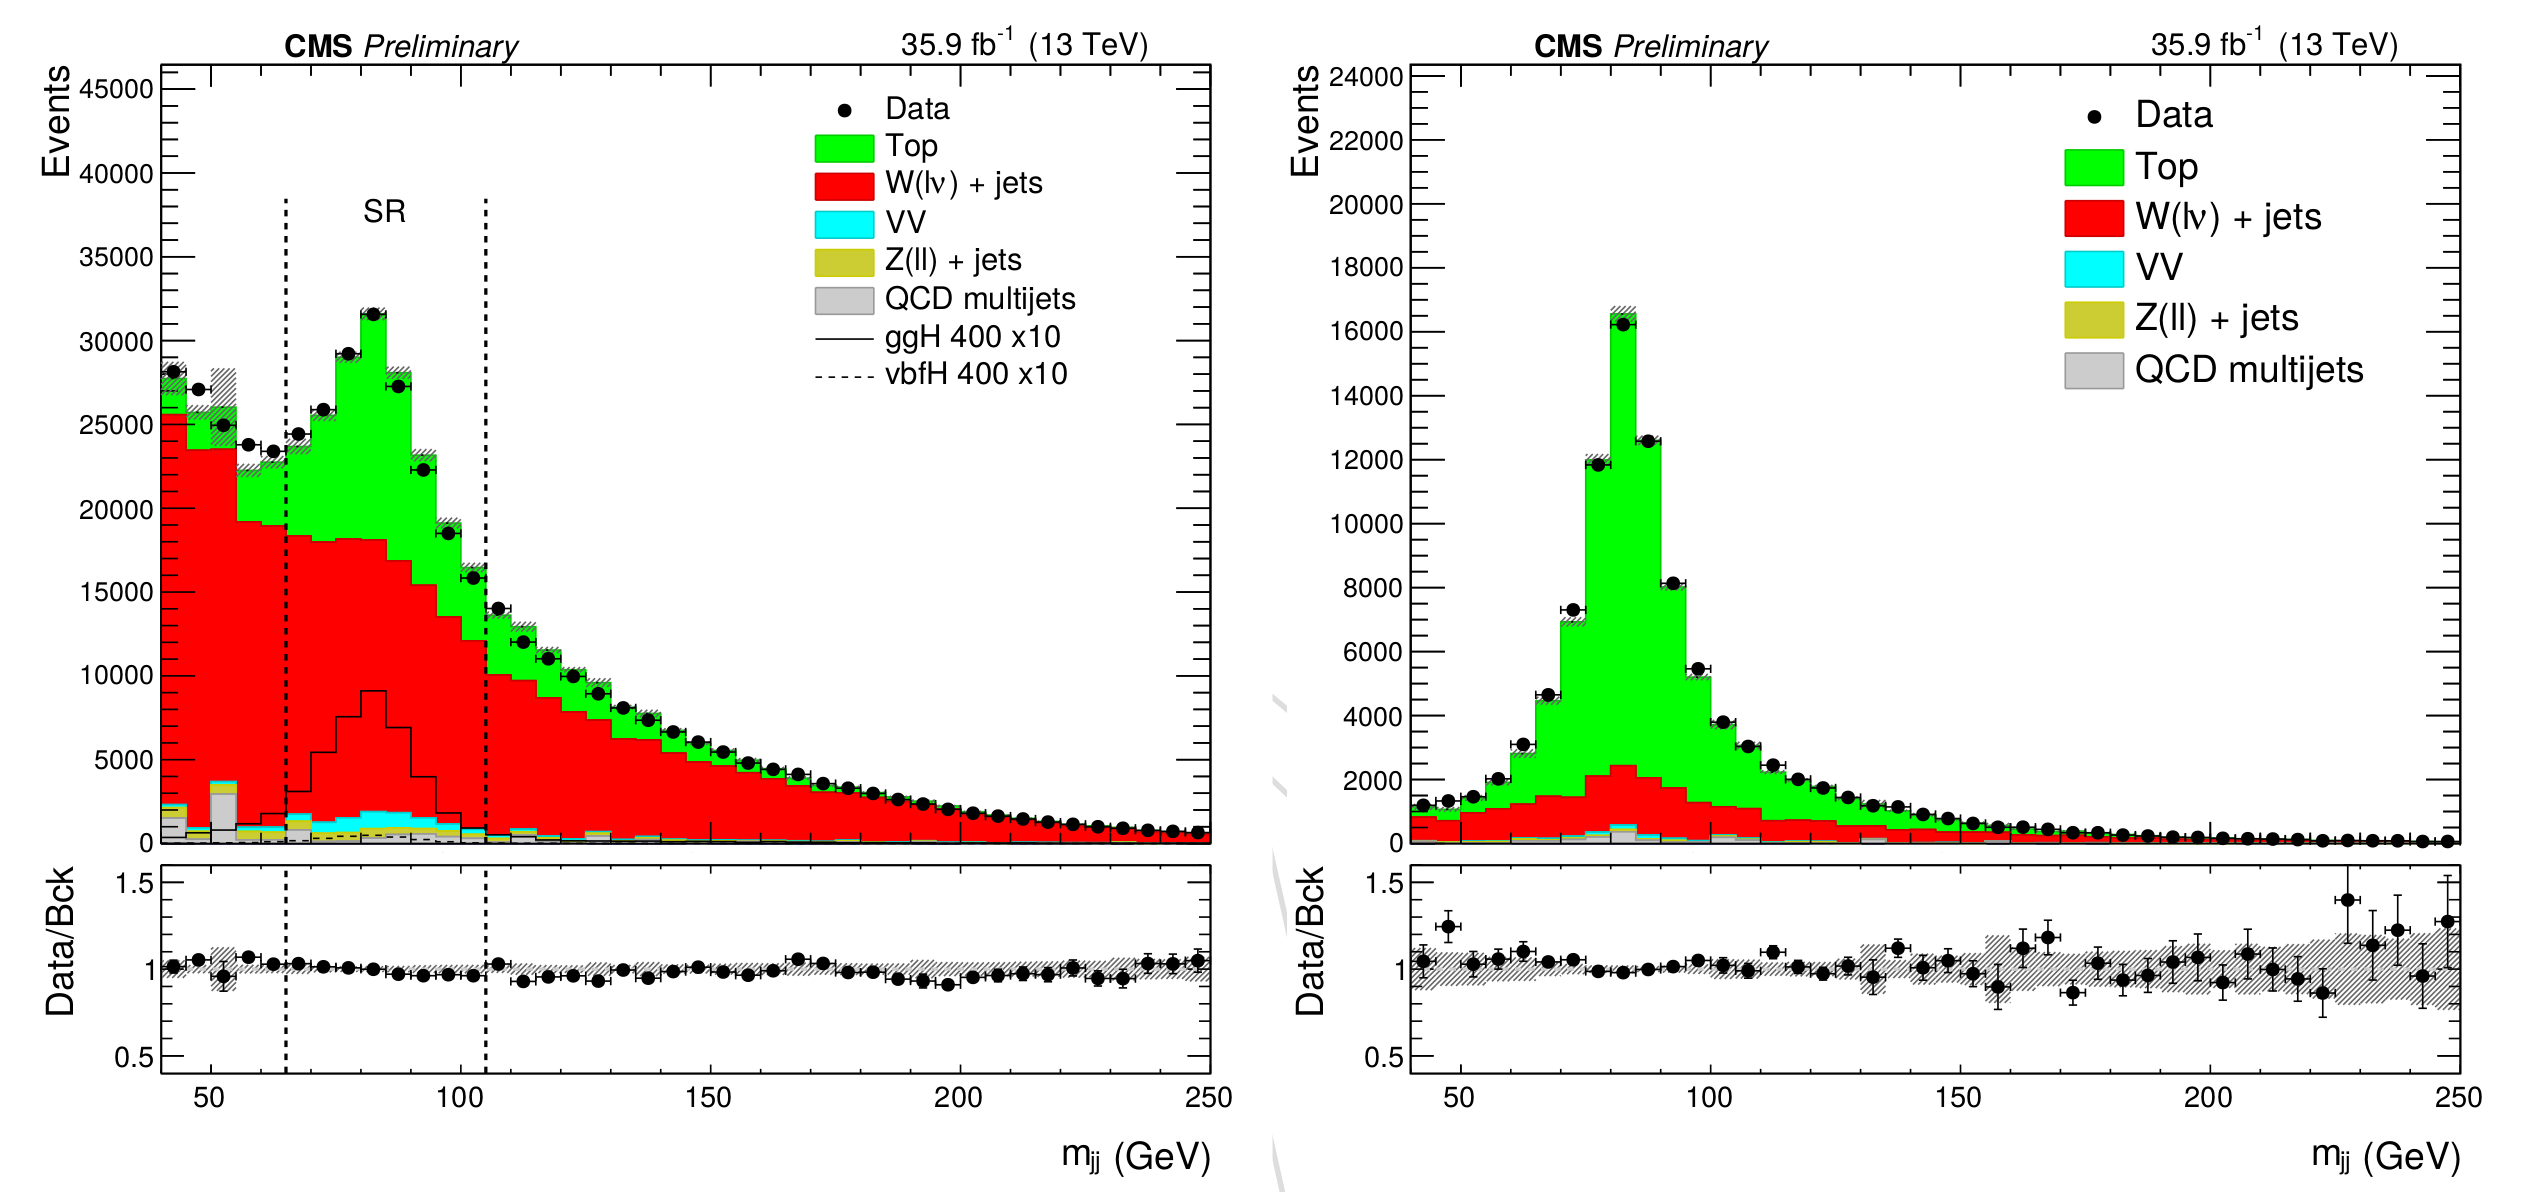
\includegraphics[scale= 0.8]{../Cap5/mjj}
\caption{Hadronic W dijet mass in data and simulation for events passing the resolved selection in the SR and SB (left), and the Top CR (right).}
\label{mjj}
\end{figure}



\section{Event categorisation}
In this analysis the events are categorised by the flavour of the lepton (electron and muon)
and type of hadronic W candidate (boosted and resolved). To increase the signal sensitivity
further we also divide events into categories based on the tagging of VBF  production and
gluon-gluon fusion for the high mass $X$ production:
\begin{itemize}
\item {\bf The VBF category}: for the identification of a VBF high mass candidate event, it is required two additional AK4 jets
with $p_T>$ 30 GeV and $\eta <$ 4.7. If there are more then two additional jets then the pair with
the highest invariant mass is chosen. An event enters the VBF category if the dijet pair has a
separation in $\eta$ ,  $\Delta \eta_{jj}$ , greater than 3.5 and an invariant mass, $m_{jj}$ , greater than 500 GeV.
\item {\bf The gluon-gluon fusion category}: those events which are not tagged as VBF selection are considered for the gluon-gluon fusion category. 
The tagging of gluon-gluon fusion  is achieved
using a kinematic discriminant based on the angular distributions of the X candidate decays
products. A kinematic discriminant is constructed as :
\begin{equation}
KD=(1+\frac{c \cdot P_{Bkgr}}{P_{Sig}})^{-1} \: , \end{equation}
where $c$ is a that  may be tuned to adjust the relative normalisations of probabilities. 
$ P_{Bkgr}$ and $P_{Sig}$  are the probability for an event to come from either background or signal respectively calculated using JHUG EN and MCFM.
The discriminant is continuously distributed between 0 and 1, with signal being closer to 1 and background closer to 0. 
In this analysis a cut at 0.5 is used to tag gluon-gluon fusion.
\item {\bf The untagged category}: events failing the   kinematic discriminant requirement  gluon-gluon fusion category and the  VBF category 
enter the untagged category.
\end{itemize}
Since the decay products of the spin-0 resonance can be fully reconstructed, it is possible to use
the reconstructed resonance mass distribution to discriminate signal events from background
events. The reconstructed mass will peak around the true resonance mass, $m_X$, for the signal,
while for background processes it will have a broader distribution.\\ 
\newline
The $m_{\ell \nu J}$ and $m_{\ell \nu jj}$ mass distributions in the singnal region, for the three categories (untagged,gluon-gluon fusion and VBF ) 
are depicted in Fig.~\ref{SR}. 
The mass distributions are compared to the background
predictions after fitting to the data in the SR with the SB and Top CR used to constrain the
background normalisations. 
\begin{figure}[htbp]
\centering
\subfigure[$m_{\ell \nu J}$]{
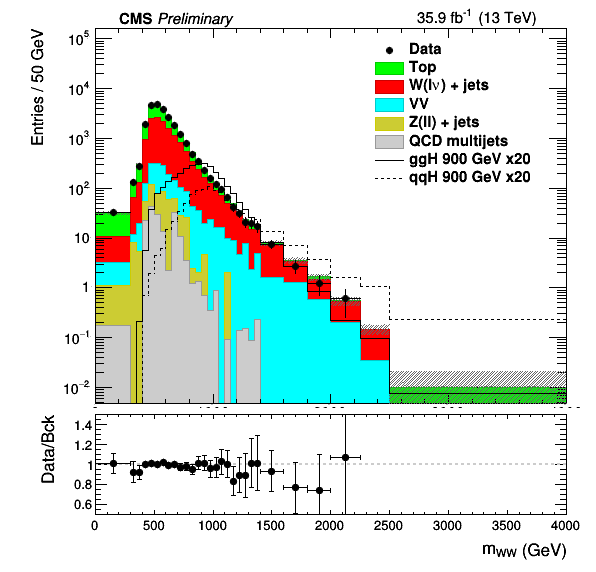
\includegraphics[width=0.45\textwidth]{../Cap5/fit_b_BoostedGG0SR_All_Log}
}
\subfigure[ $m_{\ell \nu jj}$]{
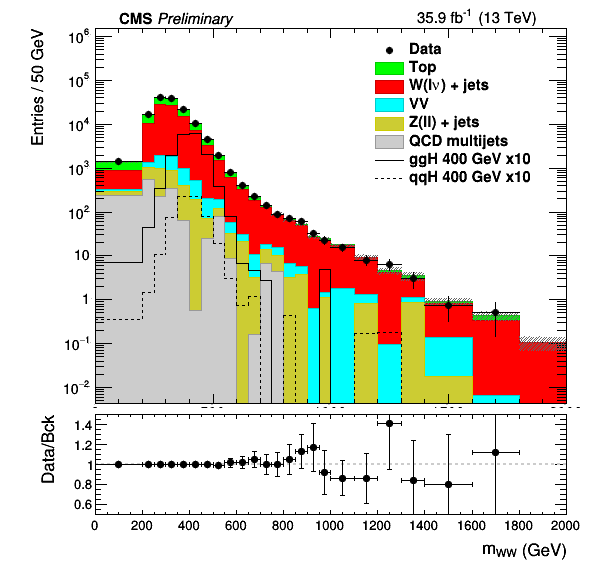
\includegraphics[width=0.45\textwidth]{../Cap5/fit_b_ResolvedGG0SR_All_Log}
}                                              
\\                                             
\subfigure[$m_{\ell \nu J}$]{                             
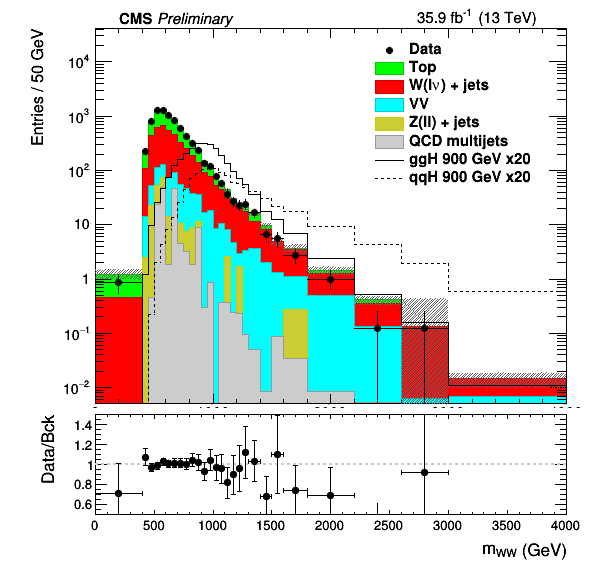
\includegraphics[width=0.45\textwidth]{../Cap5/fit_b_BoostedGG1SR_All_Log}
}                                              
\subfigure[ $m_{\ell \nu jj}$]{                               
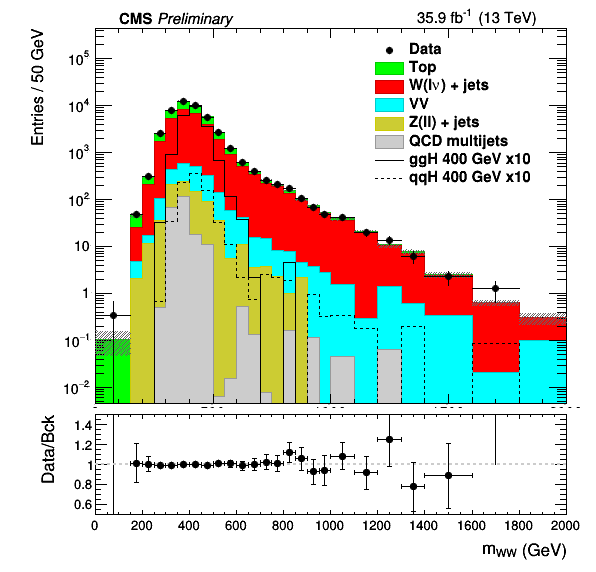
\includegraphics[width=0.45\textwidth]{../Cap5/fit_b_ResolvedGG1SR_All_Log}
}\\

\subfigure[$m_{\ell \nu J}$]{                             
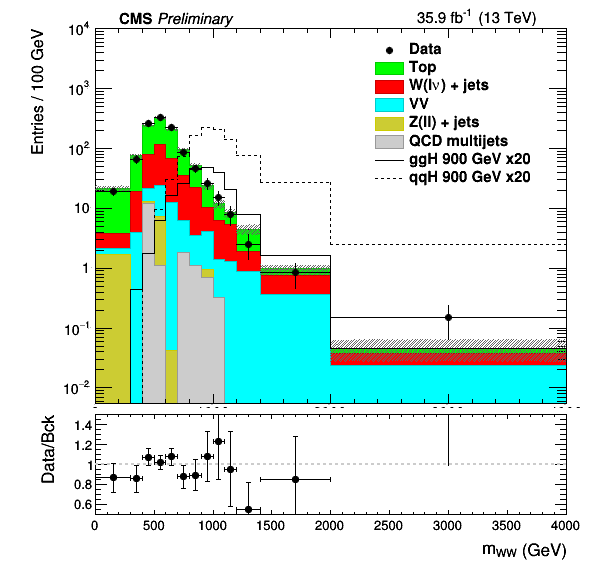
\includegraphics[width=0.45\textwidth]{../Cap5/Fit_b_BoostedVBFSR_All_Log}
}                                              
\subfigure[ $m_{\ell \nu jj}$]{                               
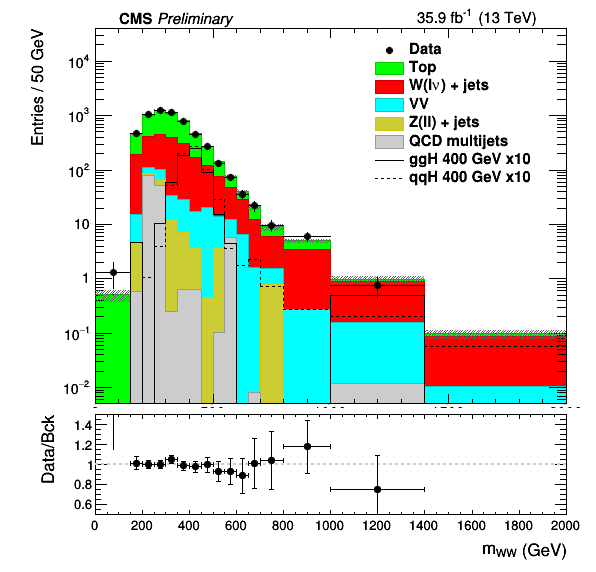
\includegraphics[width=0.45\textwidth]{../Cap5/fit_b_ResolvedVBFSR_All_Log}
}\\

\caption{The $m_{\ell \nu J}$ distribution in boosted  selection on the left, and $m_{\ell \nu jj}$ distribution in resolved selection on the right for  data and for simulation for events passing the SR selections in the untagged (top), gluon-glion fusion (middle) and VBF categories (bottom). 
The W+jets and top background normalisations  are taken from a fit to the data in the SR, SB and Top CR.}
    \label{SR}
\end{figure}

\section{Backgrounds}
The main backgrounds in this analysis are from $W$+jets and top production. Sub-dominant
backgrounds considered are SM diboson production, $Z$+Jets and QCD multijet production.
Background samples are modeled by MC simulation that has been properly reweighted to
account for known discrepancies between data and simulated events.
The boosted V tagging efficiency data-to-MC scale factor of 1.0 $\pm$ 0.06 
and is applied to diboson events satisfying the final selection cuts. 
The QCD multijet background is greatly suppressed in this analysis and is estimated with \PYTHIA.
Most events in the selected sample come from $W$+jets and top production. 
The \MADGRAPH is used to describe the contribution from W+jets, $t \bar{t}$ and single top s-channel production
while \POWHEG is used for single top t-channel and tW-channel production. 
A good level of agreement between data and simulation is demonstrated by the SR, SB and Top CR distributions.
For the final analysis, the W+jets and top X candidate mass distributions  are extracted from the simulation. 
However in each category an alternative normalization to that predicted by the MC is allowed. 
The normalization of each background is parametrized by a
multiplicative factor that is allowed to float free in the fits to the data and is constrained by the
observed yields in the SR, SB and Top CR.

\section{Systematic uncertainties}
In this section the systematic uncertainties affecting the boosted and resolved categories are
presented:
\begin{itemize}
\item  Luminosity uncertainty:  the uncertainty on LHC luminosity is 2.5\%.
\item Subdominant background normalization: a 101\% uncertainty on the normalization of the diboson, Z+jets and QCD multijets
backgrounds is aassigned.
\item Lepton trigger, identification and isolation: Lepton trigger, reconstruction, identification and isolation scale factors have been computed
using tag-and-probe technique for both muons  and electrons. 
The scale factors are apllied in this analysis and the related uncertainties estimated by shifting up and down
the scale factors by their uncertainty. Additionally for muons flat systematic uncertainties are
assigned for the trigger (0.5\%), identification (1\%) and isolation (0.5\%). 
For electrons with $p_T>$ 80 GeV a flat systematic uncertainty of 1\% is also assigned to the reconstruction. The total
uncertainty for muons is 1.5\%, while for electrons it is 2.9\%.
\item Lepton energy scale: Uncertainties related to the lepton energy scale are small. The effect on normalisation
is found to be around 0.5\%.
\item Jet energy scale and resolution: uncertainties related to the jet energy scale are calculated by changing the jet energies by $\pm$ 1
sigma error of the corresponding jet energy corrections for AK8 and AK4 jets.
Uncertainties related to the jet energy resolution are accessed by applying the recommended
resolution scale factors, which typically have a value of 1.1, and comparing the result with
the central analysis. The variations in jet energy scale and resolution are also propagated to the
MET measurement.
\item Heavy quark flavor tagging uncertaint: the uncertainties related to the b-tagging efficiency of b-jets and to the mistag probability of
light jets has been estimated by independently varying the corresponding data-to-Monte Carlo
scale factors  by one sigma, as a function of $p_T$ and $\eta$ of the jets.
\item Boosted V tagging efficiency uncertainty: the uncertainty related to the boosted V tagging efficiency for signal, top and diboson background 
events has been estimated  as data-to-Monte Carlo scale factor uncertainty of 6\% for the selection cuts. 
\item Boosted V mass scale and resolution uncertainties: the PUPPI softdrop mass scale (JMS)  and resolution (JMR) have been measured using boosted
W bosons from top decays. For signal and backgrounds containing hadronic W decays, uncertainties 
related to the JMS and JMR have been estimated by varying the mass and resolution
calibrations within their measured uncertainties.
As there are no corresponding calibration
measurements for QCD jets we treat the JMS and JMR measurements for boosted W events as
a standard candle. For those backgounds containing QCD jets we apply JMS and JMR uncer-
tainties based on varying the mass and resolution by the measured uncertainties for boosted
W events. These uncertainties are found to have a negligible effect on the $m_{\ell \nu J}$ and $m_{\ell \nu jj}$ shapes
and so are treated as normalisation systematics only.
\end{itemize}
